\documentclass[convert = false]{standalone}
\usepackage[dvipsnames]{xcolor}
\usepackage{tikz}
\usetikzlibrary{shapes.geometric, arrows, petri, positioning, fit, backgrounds, shapes.arrows, arrows.meta, calc}

% style workflow
\tikzstyle{startstop} = [rectangle, rounded corners, minimum width=3cm, minimum height=1cm,text centered, draw=black, fill=red!30]
\tikzstyle{io} = [trapezium, trapezium left angle=70, trapezium right angle=110, minimum width=3cm, minimum height=1cm, text centered, draw=black, fill=blue!30]
\tikzstyle{process} = [rectangle, minimum width=3cm, minimum height=1cm, text centered, draw=black, fill=orange!30]
\tikzstyle{process} = [rectangle, minimum width=3cm, minimum height=1cm, text centered, draw=black, fill=orange!30]
\tikzstyle{decision} = [diamond, minimum width=3cm, minimum height=1cm, text centered, draw=black, fill=green!30]
\tikzstyle{arrow} = [thick,->,>=stealth]
\tikzstyle{submodule}=[draw, dashed, rectangle, rounded corners=2pt, minimum width=1.5cm, inner sep=10pt]

\begin{document}
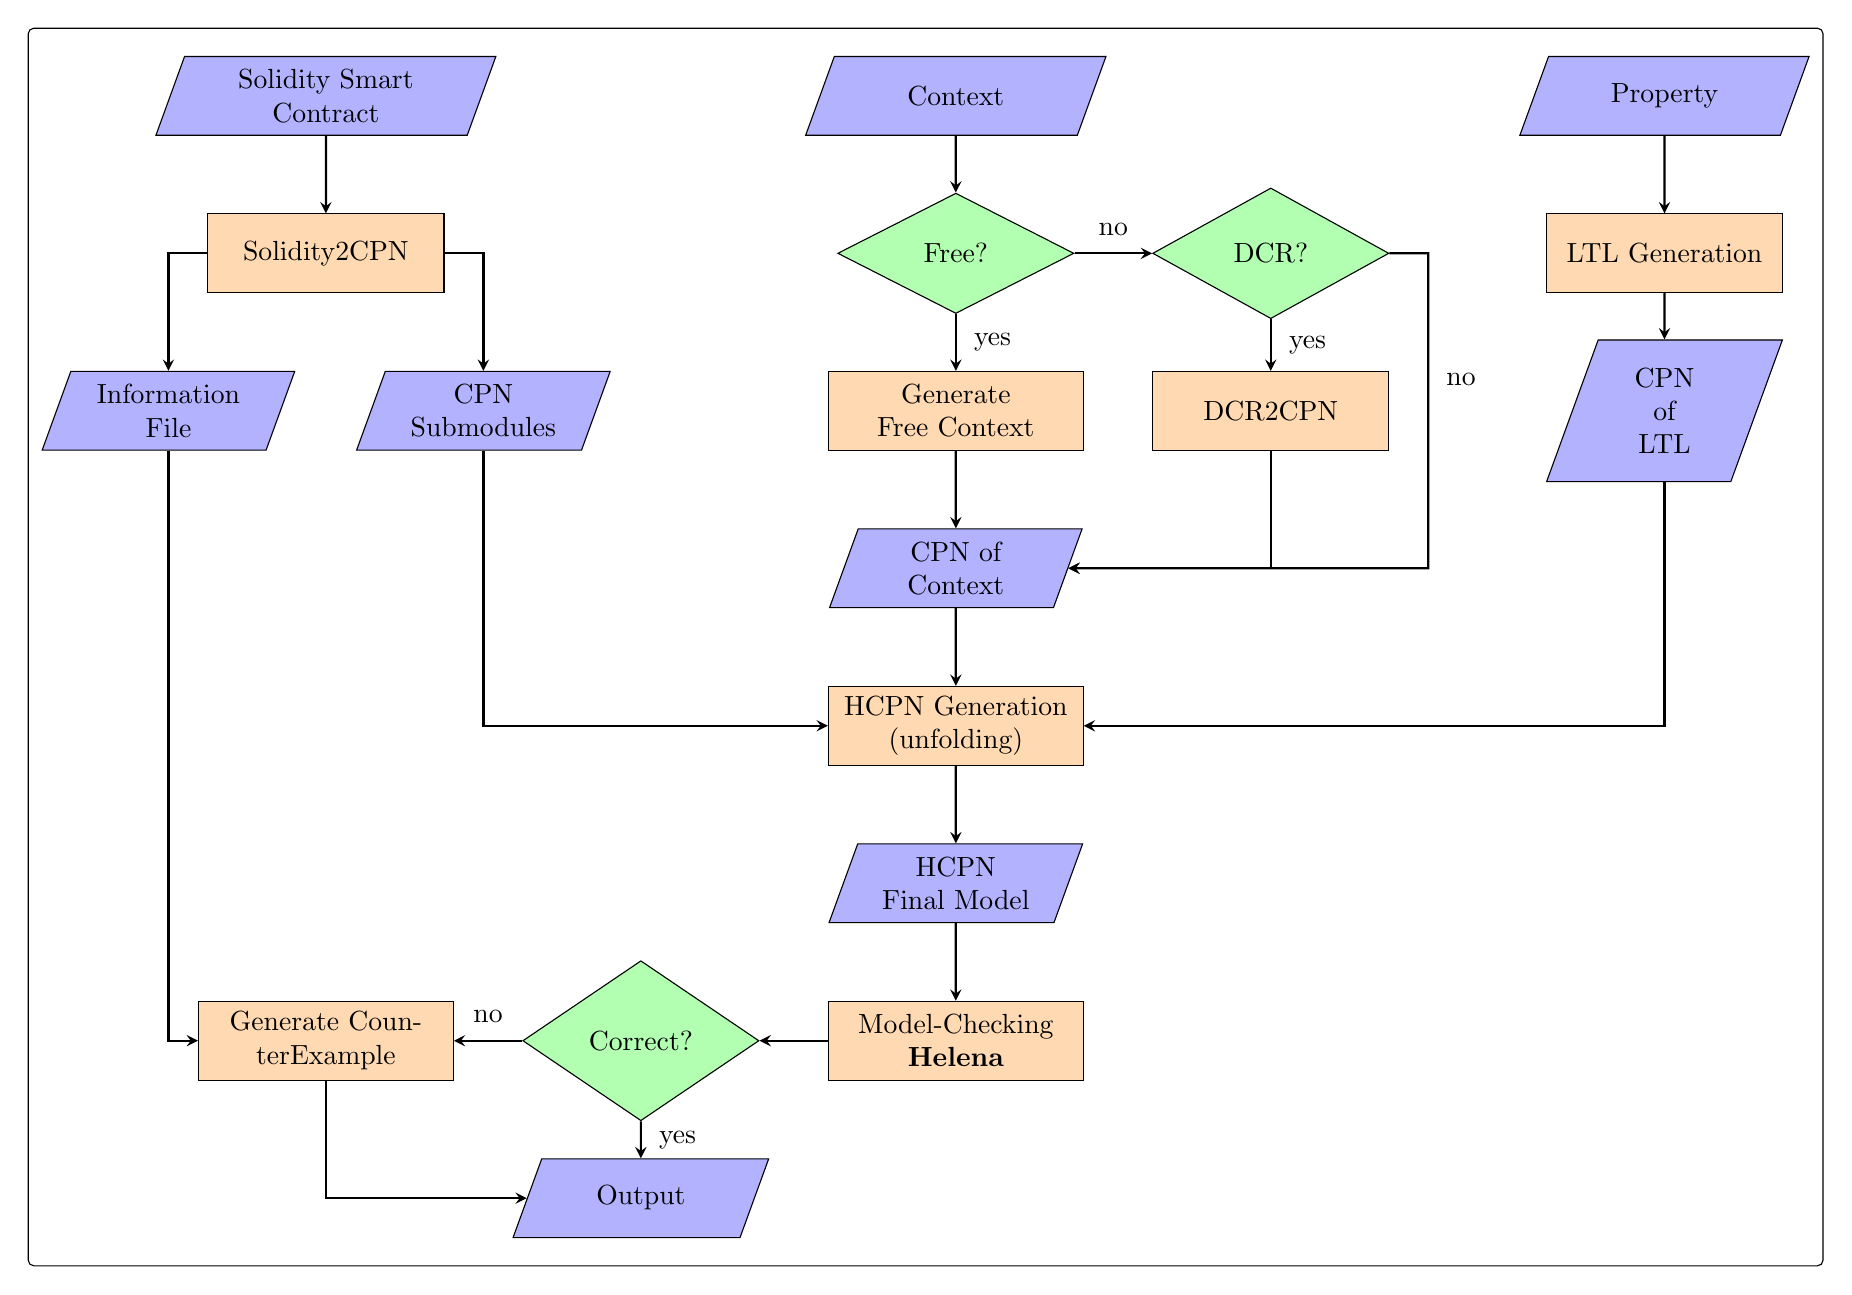
\begin{tikzpicture}[node distance=2cm]
        % context
        \node[io] (Context) {Context};
        \node[decision, below of = Context] (IsFreeContext) {Free?};
        \draw [arrow] (Context) -- (IsFreeContext);
        \node[process, below of = IsFreeContext, text width = 3cm] (GenerateFree)  {Generate Free Context};
        \node[decision, right of = IsFreeContext, xshift = 2cm] (IsDCR) {DCR?};
        \draw [arrow] (IsFreeContext) -- node[above,yshift=1mm] {no} (IsDCR);
        \draw [arrow] (IsFreeContext) -- node[right,xshift=1mm] {yes} (GenerateFree);
        \node[process, below of = IsDCR] (DCR2CPN)  {DCR2CPN};
        \draw [arrow] (IsDCR) -- node[right,xshift=1mm] {yes} (DCR2CPN);

        \node[io, below of = GenerateFree, text width = 2cm] (CPNOfContext)  {CPN of Context};

        % smart contract
        \node[io, left of = Context, xshift = -6cm, text width = 3cm] (SC)  {Solidity Smart Contract};
        \node[process, below of = SC] (S2CPN)  {Solidity2CPN};
        \draw [arrow] (SC) -- (S2CPN);

        \node[io, below of = S2CPN, xshift=2cm, text width = 2cm] (CPNModel)  {CPN Submodules};
        \draw [arrow] (S2CPN) -| (CPNModel);

        \node[io, below of = S2CPN, xshift=-2cm, text width = 2cm] (S2CPNJSON)  {Information File};
        \draw [arrow] (S2CPN) -| (S2CPNJSON);

        % property
        \node[io, right of = Context, xshift = 7cm] (Property)  {Property};
        \node[process, below of = Property] (LTLGeneration)  {LTL Generation};
        \node[io, below of = LTLGeneration, text width=1cm] (CPNLTL) {CPN of LTL};
        \draw [arrow] (Property) -- (LTLGeneration);
        \draw [arrow] (LTLGeneration) -- (CPNLTL);

        % unfolding
        \node[process, below of = CPNOfContext, text width = 3cm ] (unfolding)  {HCPN Generation (unfolding)};
        \draw [arrow] (IsDCR) -| node[right, xshift=1mm, pos=.7] {no} ($(CPNOfContext) + (6cm,0)$) -- (CPNOfContext);
        \draw [arrow] (GenerateFree) -- (CPNOfContext);
        \draw [arrow] (CPNOfContext) -- (unfolding);
        \draw [arrow] (DCR2CPN) |- (CPNOfContext);
        \draw [arrow] (CPNModel) |- (unfolding);
        \draw [arrow] (CPNLTL) |- (unfolding);

        \node[io, below of = unfolding, text width = 2cm] (FinalModel) {HCPN Final Model};
        \draw [arrow] (unfolding) -- (FinalModel);

        % model checking
        \node[process, below of = FinalModel, text width = 3cm] (MC) {Model-Checking \textbf{Helena}};
        \draw [arrow] (FinalModel) -- (MC);

        \node[decision, left of = MC, xshift=-2cm] (IsCorrect) {Correct?};
        \node[process, left of = IsCorrect, text width = 3cm, xshift=-2cm] (GenerateCE)  {Generate CounterExample};
        \draw [arrow] (MC) -- (IsCorrect);
        \draw [arrow] (IsCorrect) -- node[above,yshift=1mm] {no} (GenerateCE);

        \node[io, below of = IsCorrect] (Output)  {Output};
        \draw [arrow] (IsCorrect) -- node[right,xshift=1mm] {yes} (Output);
        \draw [arrow] (GenerateCE) |- (Output);
        \draw [arrow] (S2CPNJSON) |- (GenerateCE);


            \begin{pgfonlayer}{background}
                \node[submodule, solid, fill=white, fit=(Output) (SC) (Property) (S2CPNJSON)] (MC) {};
            \end{pgfonlayer}
    \end{tikzpicture}
\end{document}